\documentclass{legrand}
\usepackage{thesis_98_packages}

%-------------------------------------------------------------------------------
%	SETTING UP SOME VARIABLES :D
%-------------------------------------------------------------------------------
\def\mytitle{Analysis and implementation of an algorithm to validate Knowledge Graphs using Big data techniques} % Title of the project
\def\subtitle{A Profound Subtitle} % Subtitle of the project
\def\centre{Escuela de Ingeniería Informática} % The name of the centre you're sitting at
\def\reviewer{Jose Emilio Labra Gayo} % reviewer of the project
\def\author{Ángel Iglesias Préstamo} % Your name.. 
\def\date{\today} % Today's date 
%-------------------------------------------------------------------------------
%-------------------------------------------------------------------------------

\begin{document}

% Uncomment and fill out to include PDF metadata for the author and title of the book
\hypersetup{
    pdftitle={\mytitle},
    pdfauthor={\author}
}

\pagenumbering{roman}

% custom commands for use in the paper
% creating some commands for reuse later on :D
\newcommand{\myfont}[1]{\ensuremath{\mathcal{#1}}}

\newcommand{\VertSet}{\myfont{V}}
\newcommand{\NodeSet}{\myfont{N}}
\newcommand{\EdgeSet}{\myfont{E}}
\newcommand{\LabelSet}{\myfont{L}}
\newcommand{\PLabelSet}{\myfont{T}}
\newcommand{\MsgSet}{\myfont{M}}
\newcommand{\None}{\myfont{None}}

\newcommand{\triple}[3]{\ensuremath{\langle #1,#2,#3 \rangle}}
\newcommand{\quadruple}[4]{\ensuremath{\langle #1,#2,#3,#4\rangle}}
\newcommand{\ItemSet}{\myfont{Q}}
\newcommand{\PropSet}{\myfont{P}}
\newcommand{\EntitySet}{\myfont{E}}
\newcommand{\ValueSet}{\myfont{V}}
\newcommand{\DataValueSet}{\myfont{D}}
\newcommand{\StmtSet}{\rho}
\newcommand{\FinSet}[1]{\ensuremath{FinSet(#1)}}
\newcommand{\Graph}{\myfont{G}}

\newcommand{\hrefc}[3][blue]{\href{#2}{\color{#1}{#3}}}%
\newcommand{\elemento}[2]{\ensuremath{\hrefc[violet]{http://www.wikidata.org/entity/#2}{#1}}}
\newcommand{\propiedad}[2]{\ensuremath{\hrefc[blue]{http://www.wikidata.org/entity/#2}{#1}}}
\newcommand{\alanTuring}{\elemento{alanTuring}{Q7251}}
\newcommand{\wilmslow}{\elemento{wilmslow}{Q2011497}}
\newcommand{\town}{\elemento{town}{Q3957}}
\newcommand{\government}{\elemento{government}{Q220798}}
\newcommand{\warringtonLodge}{\elemento{warringtonLodge}{Q20895942}}
\newcommand{\bombe}{\elemento{bombe}{Q480476}}
\newcommand{\unitedKingdom}{\elemento{unitedKingdom}{Q145}}
\newcommand{\computer}{\elemento{computer}{Q11742076}}
\newcommand{\dateOfBirth}{\propiedad{dateOfBirth}{P569}}
\newcommand{\placeOfBirth}{\propiedad{placeOfBirth}{P19}}
\newcommand{\country}{\propiedad{country}{P27}}
\newcommand{\employer}{\propiedad{employer}{P108}}
\newcommand{\discoverer}{\propiedad{discoverer}{P61}}
\newcommand{\dateOfDeath}{\propiedad{dateOfDeath}{P570}}
\newcommand{\placeOfDeath}{\propiedad{placeOfDeath}{P20}}
\newcommand{\timeStart}{\propiedad{timeStart}{P580}}
\newcommand{\timeEnd}{\propiedad{timeEnd}{P582}}
\newcommand{\manufacturer}{\propiedad{manufacturer}{P176}}
\newcommand{\Human}{\elemento{Human}{Q5}}
\newcommand{\instanceOf}{\propiedad{instanceOf}{P31}}

\newcommand{\fb}[1]{\dofb#1}
\newcommand{\dofb}[1]{\textbf{#1}\nobreak\hspace{0pt}}

\newcommand{\mi}[1]{\ensuremath{\mathit{#1}}}

\newcommand{\emptyGraph}{\ensuremath{\emptyset}}
\newcommand{\EmptyGraph}{\ensuremath{\emptyset}}
\newcommand{\addTriple}{\ensuremath{\rtimes}}
\newcommand{\unionGraphs}{\ensuremath{\cup}}
\newcommand\neighs[2]{\ensuremath{neighs(#1,#2)}}
\newcommand\nodes[1]{\ensuremath{nodes(#1)}}
\newcommand{\node}{\mi{n}}
\newcommand{\lbl}{\mi{l}}
\newcommand{\g}{\mi{g}}
\newcommand{\vertex}{\mi{v}}
\newcommand{\msg}{\mi{msg}}
\newcommand{\msgs}{\mi{msgs}}
\newcommand{\labels}{\mi{labels}}
\newcommand{\TripleConstraint}{\mi{TripleConstraint}}
\newcommand{\ShapeReference}{\mi{ShapeReference}}
\newcommand{\ShapeAnd}{\mi{ShapeAnd}}
\newcommand{\ShapeOr}{\mi{ShapeOr}}
\newcommand{\Cardinality}{\mi{Cardinality}}

% Algorithmic definitions
\SetKwProg{Def}{def}{$\,$:}{}
\SetKwProg{Defn}{def}{~$=$}{}
\SetKw{defn}{def}
\newcommand{\DefInline}[2]{\defn #1 = #2}
\SetKwProg{DefnCustom}{\defn}{}{}
\SetKw{Let}{let}
\SetKwInput{KwIn}{Input}
\SetKwFor{ForEach}{foreach}{}{}
\SetKw{Or}{or}
\SetKw{And}{and}
\SetKwIF{If}{ElseIf}{Else}{if}{then}{else if}{else}{endif}
\SetKw{Match}{match}
\SetKw{MyIf}{if}
\SetKw{MyThen}{then}
\SetKw{MyElse}{else}
\SetKw{Case}{case}
\SetKwBlock{Let}{let}{in}
\SetKw{In}{in}
\SetKw{MapTo}{\ensuremath{\;\;\Rightarrow\;\;}}
\SetKwBlock{Block}{}{}
\newcommand{\assign}{\ensuremath{~\mathtt{:=}~}}
\newcommand{\algocomment}[1]{\text{//$\,$#1}}

\newcommand{\blockskip}{\smallskip}
\newcommand{\done}{\ensuremath{\mathit{done}}}

% [algorithm spacing:]
\def\algorithmsize{small}
\def\algorithmheadersize{\algorithmsize}
\renewcommand\AlCapFnt{\normalfont\bfseries\small}
\setlength{\textfloatsep}{1.0ex}
\setlength{\floatsep}{1.0ex}

% Statuses
\newcommand{\Ok}{\ensuremath{Ok}}
\newcommand{\Failed}{\ensuremath{Failed}}
\newcommand{\WaitingFor}[3]{\ensuremath{WaitingFor}(#1,#2,#3)}
\newcommand{\Pending}{\ensuremath{Pending}}
\newcommand{\PendingLs}{\ensuremath{Pending}(ls)}
\newcommand{\Undefined}{\ensuremath{Undefined}}

\newcommand{\Validate}{\ensuremath{Validate}}
\newcommand{\Checked}[2]{\ensuremath{Checked(#1,#2)}}
\newcommand{\WaitFor}[1]{\ensuremath{WaitFor(#1)}}
\newcommand{\status}[2]{\ensuremath{#1(#2)}}
\newcommand{\msgSent}[3]{\ensuremath{#1,#2\rightsquigarrow{}#3}}
\newcommand{\checkLocal}[2]{\ensuremath{checkLocal(#1,#2)}}
\newcommand{\checkLocalOpen}[2]{\ensuremath{checkLocalOpen(#1,#2)}}

\newcommand{\neighbors}[3]{\ensuremath{neighbors}(#1,#2,#3)}
\newcommand{\fracEmpty}[2]{\genfrac{}{}{0pt}{0}{#1}{#2}}
\newcommand{\vProg}{vProg}
\newcommand{\tripleConstraints}[1]{tripleConstraints(#1)}
\newcommand{\rbe}[1]{\ensuremath{rbe(#1)}}
\newcommand{\combine}[2]{\ensuremath{combine(#1,#2)}}

\chapterimage{img/misc/heading_main.pdf} % Chapter heading image

% make title out of \author, \title, \date  specified in the preamble
\begingroup
\thispagestyle{empty}
\begin{tikzpicture}[remember picture,overlay]
    \coordinate [below=10cm] (midpoint) at (current page.north);
    \node at (current page.north west)
    {\begin{tikzpicture}[remember picture,overlay]
            \node[anchor=north west,inner sep=0pt] at (0,0) {
\includegraphics[width=\paperwidth]{img/cover_bg}}; % Background image
            \draw[anchor=north] (midpoint) node [fill=blueUniovi!30!white,fill opacity=0.6,text opacity=1,inner sep=1cm, text width=21cm, minimum width=\paperwidth]
            {\Huge\centering\bfseries\sffamily\parbox[c][][t]{\paperwidth}
            {\centering\mytitle\\[15pt] % Book title
            {\Large\subtitle}\\[20pt] % Subtitle
            {\huge\author}\\[1pt] % Author's name
            {\large Supervised by \textit{\reviewer}} % Reviewer's name
            }};
        \end{tikzpicture}};
\end{tikzpicture}
\vfill
\endgroup

% include the abstract, written in a separate file called thesis_02_abstract.tex
\setcounter{page}{0}
\newenvironment{abstract}%
{\cleardoublepage\null\vfill\section*{\abstractname}}%
{\vfill\null}
\begin{abstract}
    The necessity of processing large amounts of data is getting increased with time. Not only we do need to process high volumes of sequential information, but more complex structures such as graphs. As an example of that, one of the sources we can retrieve data from is Wikidata, the central storage for the structured data of Wikimedia projects: including Wikipedia. The shape of the documents to be processed from Wikidata tends to be heterogeneous: the structure of a human node may vary from the one of a mountain. More in more, it could be helpful to generate subsets out of a dump for us to work only with concrete nodes.

    Not only that but, the last tendencies in \textit{data integration} show that the data is not only stored in a single place but distributed among different sources. This is the case of biological data where several different databases are used to store the information, including \texttt{Uniprot} and \texttt{PubChem}. The data is stored in different formats, and it is not always easy to integrate it. However, through \textit{subsets} we can create a common ground for the data to be processed. This is, we can create a subset of the data that is common to all the sources, and then process it.
\end{abstract}

\noindent \textbf{Keywords} --- \textit{Knowledge Graphs, RDF, Linked Data, RDF Validation, Shape Expressions, Subsets, MapReduce, Pregel, Algorithms, Wikibase, Apache Spark, Scala, Rust, DuckDB.}
\phantom{~}

\vfill

\begin{flushright}
    {\em
        Data is a precious thing\\[0.25\baselineskip]
        and will last longer than the systems themselves\\[1.5\baselineskip]
        --Tim Berners-Lee
    }
\end{flushright}

\bigskip

\begingroup

\let\clearpage\relax
\let\cleardoublepage\relax
\let\cleardoublepage\relax

\section*{Acknowledgements}

\noindent Put your acknowledgements here.

\endgroup

\vfill

% Create table of contents - not mandatory
\pdfbookmark{\contentsname}{toc}
\tableofcontents

% Create a list of figures
\listoffigures

% Create a list of tables
\listoftables


\chapter{Introduction}
% and we establish the numeration back to the normal one 
\setcounter{page}{0} % reset numbering to 1, 2, 3...
\pagenumbering{arabic}
\label{chapter:intro}
\epigraph{\textit{We cannot solve problems with the kind of thinking we employed when we came up with them.}}{-- \textup{Albert Einstein}}

During the following paragraphs I am covering the motivation, contributions and structure of this document. This means, after reading it, you are building the big picture; a general idea of the motivations to develop this project, the results we are looking for and the shape of it.

\section{Motivation}

These days, more and more devices are connected among them. Not only that, but tons of information is being stored automatically. This makes the task of having to process that data a more complex job. What's more, it is also becoming a more relevant assignment. Simply stated, the amount of data outruns our capacity to consume it.

A solution to that is Big data: an emerging field of Software development where we process strong volumes of diverse information at a speed. Big data applications not only have to scan large amounts of inputs the faster they can, but the variety of sources that information comes from makes interoperability a key concept we must deal with.

Knowledge graphs~\cite{https://doi.org/10.48550/arxiv.2110.11709} were popularized back in 2012 by Google~\cite{web:knowledge_graphs:google} as a tool to represent real world data reflecting relationships between entities in order to understand those links better. After Google's introduction, others embraced this approach: ranging from proprietary to open databases. Being the content of the latter publicly available. Prominent companies -- including \textit{web search} (e.g., Bing~\cite{knowledge:graphs:usage:bing} and Google~\cite{web:knowledge_graphs:google}), \textit{commerce} (e.g., Airbnb~\cite{knowledge:graphs:usage:airbnb} and Amazon~\cite{knowledge:graphs:usage:amazon}), \textit{social networks} (e.g., Facebook~\cite{knowledge:graphs:usage:facebook} and LinkedIn~\cite{knowledge:graphs:usage:linkedin}) or \textit{finances} (e.g., Accenture~\cite{knowledge:graphs:usage:accenture} and Banca d'Italia~\cite{https://doi.org/10.48550/arxiv.2010.05172}) -- are using knowledge graphs in order to have a better understanding of their customers. Even though there exist several models associated with this technology, we are focusing on wikibase graphs.

Summing up, this project focuses on the analysis and implementation of a system to validate wikibase graphs -- an specific flavour of the so-called knowledge graphs -- using big data techniques. To put that into perspective, as of October 1, 2022, a compressed dump\footnote{\textbf{dump:} is a copy of the whole Wikibase raw data that can be downloaded from their system. This could also be understood as a snapshot of what was stored in the system at a certain moment.} of Wikidata's database has a size of 109.04Gb~\cite{wikidata:dumps}. Not only that, but the size of these dumps has exponentially increased with each and every release of a new one (see figure \ref{fig:dumps}).

\begin{figure}[ht]
    \centering
    \includestandalone{figures/fig_01_dumps}
    \caption[Plot showing the size of compressed dumps between 2014-22]{Size of compressed wikidata dumps between 2014-2022~\cite{https://doi.org/10.48550/arxiv.2110.11709}}
    \label{fig:dumps}
\end{figure}

\textbf{Project's Goal 1.} \textit{Design and implementation of a system for validating huge dumps from Wikidata generating a subset out of it.} As we have stated during these introductory lines, the task of having to process enormous amounts of data is becoming increasingly relevant. The faster a system allows us to accomplish it, the better solution we will provide.

\textbf{Project's Goal 2.} \textit{Reproduce an experiment related to the analysis of the previously described algorithm.} In order us to properly analyze the results emerging from the execution of the algorithm we have implemented, we have to create an ecosystem were we can obtain information related to memory consumption or execution time, to name a few.

\textbf{Project's Goal 3.} \textit{Learn new technologies and Big data techniques.} This is an academic project, not only that, but one of the main objectives of researching is finding new solutions to a certain problem. This means, learning and exploring new possibilities is -- indeed -- one goal of this project.

\section{Contributions}

The main contributions of this project are:

\begin{enumerate}
    \item
\end{enumerate}

\section{Structure of the document}

The shape of this document is as follows:

\begin{itemize}
    \item \textbf{Chapter ~\ref{chapter:description}.} General description of the existing technologies related to knowledge graph validation. As well as the advantages and disadvantages of choosing some tools over others for implementing this project.
    \item \textbf{Chapter ~\ref{chapter:theory}.} Provides a theoretical background needed for better understanding the concepts explained in the following chapters.
    \item \textbf{Chapter ~\ref{chapter:experiment}.} Explanation of the process followed to analyze the concrete implementation of the algorithm that we used to validate the knowledge graphs.
    \item \textbf{Chapter ~\ref{chapter:results}.} Analysis of the results obtained from the previously described experiment.
    \item \textbf{Chapter ~\ref{chapter:conclusions}.} Summary of the general conclusions and future work.
\end{itemize}

\chapter{Related Work}
\label{chapter:related}
\epigraph{\textit{If I have seen further, it is by standing on the shoulders of giants.}}{-- \textup{Isaac Newton}}

Some work has already been done in the field of Knowledge graph validation. In this section we are exploring what other projects have achieved and their limitations.

\section{Bid data processing and graphs}

Having to process enormous graphs made Google propose Pregel~\cite{10.1145/1807167.1807184} a model for large-scale graph computing, back in 2010. Following the idea of \textit{think like a vertex}, other systems were introduced: GraphLab~\cite{10.14778/2212351.2212354}, PowerGraph~\cite{180251} or GraphX~\cite{186216}. Being the latter a framework that enables the implementation of parallel computing algorithms.

\section{Knowledge graphs}

This article is closely related to Labra's paper~\cite{https://doi.org/10.48550/arxiv.2110.11709} on utilizing Shape Expressions to generate knowledge graph subsets, where he described the approach used in this document as one of the potential implementations. MARS (Multi-Attributed Relational Structures)~\cite{ijcai2017p165}, which are a generalized concept of property graphs, are the source of inspiration for our description of Wikibase graphs. They also define MAPL (Multi-Attributed Predicate Logic) as a formalism of logic that may be applied to ontological reasoning in that work.

\section{Knowledge graph descriptions}

\section{Knowledge graph subsets}

\chapter{Theoretical Background}
\label{chapter:theory}
\epigraph{\textit{It doesn't matter how beautiful your theory is, it doesn't matter how smart you are. If it doesn't agree with experiment, it's wrong.}}{-- \textup{Richard P. Feynman }}

\section{Knowledge graph}

A knowledge graph uses a graph-structured data model to represent knowledge of some real world domain. Where each node represents an entity and the edges are the relationships between them. These graphs can be represented using different technologies; however, we will focus on attributed graphs.

\subsection{Wikibase graphs}

Wikibase graphs are the main example of attributed ones, where we can represent property-value pairs

\section{Data-flow algorithms}

The main focus of this document is implementing a Big data solution using the Pregel algorithm. However, for better understanding it, introducing the MapReduce model will be handful. Notice that both are meant to be executed in parallel in a distributed system.

\subsection{MapReduce}

Inspired by the map and reduce functions, a MapReduce~\cite{wiki:MapReduce} program is composed of a \textit{map procedure}, where we apply a simple operation to all the elements of a sequence, followed by a \textit{reduce} method, which transforms those elements into a single result. For us to process a graph, we would need to chain MapReduce invocations. Where, for each iteration, map and reduce functions are applied. The main drawback of this approach, is the functional nature of the MapReduce model. This means, expressing a graph algorithm as a chained MapReduce results in having to pass the entire state of the graph from one stage to another~\cite{10.1145/1807167.1807184} .

\subsection{Pregel model}

Pregel (\textit{Parallel, Graph and Google}) is a data flow paradigm and system created by Google to handle large-scale graphs. Even though the original system remains proprietary at Google, the computational model was adopted by many graph-processing systems: including Apache Spark. For better understanding Pregel, the idea is to \textit{think like a vertex}; this way, for computing the state of a given node, we only depend on the states of its neighboring\footnote{We will call neighboring vertices of a certain one to those nodes connected to it by an outgoing edge.} ones. \textit{Thinking like a vertex} could be understood as the \textit{leitmotif} for dividing the problem into several sub-problems: instead of dealing with a huge graph\footnote{A graph to be processed with Pregel may potentially have millions of vertices with billions of edges. More on the size of the Wikibase graphs will be discussed later on.}, we just have to solve the problem for smaller graphs: a vertex and its neighboring ones.

In comparison to the MapReduce framework, where for each iteration the state of the whole graph must be passed, at each \textit{superstep} -- the way we refer to iterations in Pregel -- each vertex can: send a message to its neighbors, process the received messages (from the previous superstep), and update its state. Summing up, instead of sending the whole state of the graph, we just send messages back and forth. The best way for understanding this is through an example. Let me show you the resulting trace after applying Pregel for computing the maximum value in a graph (see figure \ref{fig:pregel}).

\begin{figure}[h]
    \centering
    \includestandalone{figures/pregel_trace}
    \caption[Trace of the execution of Pregel for computing the maximum value]{Trace of the execution of Pregel for computing the maximum value~\cite{10.1145/1807167.1807184}}
    \label{fig:pregel}
\end{figure}

Notice that at the beginning of the execution, the state of all the nodes will be set to active. This initial stage is called \textit{superstep 0}. When a vertex is active, it sends a message to its neighbors, that will receive it in the next \textit{superstep}. In this case, the message we are propagating is the largest value that we have learned so far. As an example to that, the second to the left node starts with a value of 6 -- which is the maximum value of the graph -- and sends that number to its neighbors: 3 and 1. In the next \textit{superstep}, the vertices that have received a message have to compare both: the value they store and the received one. This comparison is what it's called the \textit{vprog} function, which will vary from one problem to another. Then, both nodes will update its state to 6. As they have updated their state, they will have to send the new value to its neighbors: beginning another iteration (\textit{superstep}). Notice that at the \textit{superstep 1}, the second to the left node is halted as it doesn't send any other message to its neighbors as it's value has not changed. When every node is halted -- inactive -- the execution of the algorithm finishes. In the figure \ref{fig:state} a simplified state machine is shown.

\begin{figure}[h]
    \centering
    \includestandalone{figures/state_diagram}
    \caption[Simplified state diagram of a vertex]{Simplified state diagram of a vertex~\cite{10.1145/1807167.1807184}}
    \label{fig:state}
\end{figure}

\subsubsection{Architecture of a Pregel system}

It's quite simple to describe the architecture of a Pregel system. As we have seen, one of the main goals of this algorithm is achieving a parallel execution. This way, a \textit{master} node will divide the graph into several partitions and assign one (or more) of them to each \textit{worker} node. For the \textit{master} to create the partitions it selects a bunch of vertices and all those vertices' outgoing edges; remember: \textit{think like a vertex}.

\begin{figure}[h]
    \centering
    \includestandalone{figures/architecture}
    \caption[Architecture of a Pregel system]{Architecture of a Pregel system~\cite{10.1145/3349265}}
    \label{fig:architecture}
\end{figure}


\part{Design and Implementation of the Pregel solution}

\chapter{First Pregel solution}
\label{chapter:first}
\epigraph{\textit{The most important single aspect of sotware development is to be clear about what you are trying to build.}}{-- \textup{Bjarne Stroustrup}}

In this chapter, we will describe the first implementation of the Pregel solution, exposing the decisions that led to it, as well as the technical debt. This first version is part of Labra's publication \cite{https://doi.org/10.48550/arxiv.2110.11709}.

\section{Technology stack}

For us to describe the technologies used, we have to summarize the needs of the solution first. A large-scala data processing framework is required. What's more, a graph-processing library implementing a Pregel abstraction is also advisable; this way, we can focus on the algorithm for creating the subsets. Finally, it would be ideal if the stated technologies were open-source and well-maintained. Let us describe the chosen stack.

\begin{figure}[ht]
    \begin{subfigure}{.3\textwidth}
        \centering
        
\includegraphics[width=.7\linewidth]{img/7-1_scala.png}
        \caption{Scala programming language}
    \end{subfigure}%
    \hspace*{0.5em}
    \begin{subfigure}{.3\textwidth}
        \centering
        
\includegraphics[width=.7\linewidth]{img/7-2_spark.png}
        \caption{Apache Spark}
    \end{subfigure}%
    \hspace*{0.5em}
    \begin{subfigure}{.3\textwidth}
        \centering
        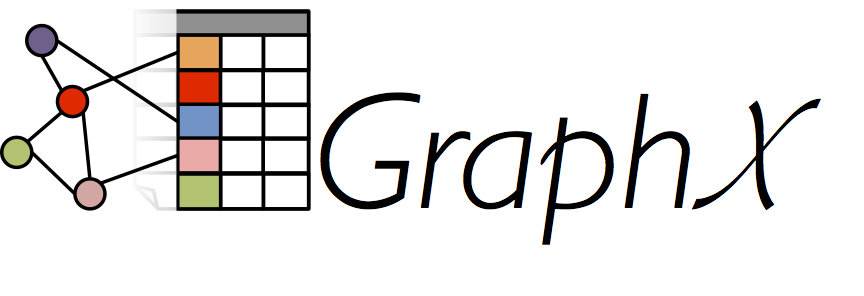
\includegraphics[width=.7\linewidth]{img/7-3_graphx.png}
        \caption{GraphX framework}
    \end{subfigure}%
    \caption{Stack of the different technologies we are using for the first solution}
\end{figure}

\subsection{Scala}

\footnotetext{\url{https://www.scala-lang.org/}}
\footnotetext{\url{https://en.wikipedia.org/wiki/Criticism_of_Java}}

Scala\footnotemark is a high-level programming language combining the object-oriented and functional paradigms. Intended to be concise and to answer the majority of Java's complaints.\footnotemark. Allowing operator overloading, a better functional support, lazy evaluation and requiring less boilerplate code. One of the features that I enjoy the most is pattern matching, which is not supported in Java. What's interesting is that Scala source code can be compiled into Java bytecode, the instruction set of the Java Virtual Machine. This way, a vast ecosystem of Java libraries are available when writing Scala programs. One of the main disadvantages of Scala is that major updates are not backwards compatible; this way, programs written in Scala 2.12 are not supported in 2.13. Not to mention that nowadays there exist two major branches of Scala development, namely Scala 2 and 3. Putting this all together, we can conclude that Scala is a bit unstable. A hell of a maintenance making loads of open-source projects and libraries get abandoned; we will discuss into this later on.

\begin{code}[Hello World written in Scala]
    \inputminted{scala}{code/listings/7-1_helloWorld.scala}
\end{code}

\subsection{Apache Spark}

Apache Spark is a Big data engine with support for several programming languages, including Scala and Python. Aiming to be simple, fast and scalable, it is the most widely-used engine in the industry. The idea behind Spark is creating a Framework that makes parallel jobs over high-volumes of data easy to write. It also bundles an engine supporting query optimization which will be discussed later on. For us to understand how Spark works, let's describe its architecture first. It follows the master-slave architecture, same idea behind the Pregel algorithm, built on top of two abstractions, namely Resilient Distributed Dataset (RDD) and Directed Acyclic Graph (DAG).

\subsubsection{RDDs (Resilient Distributed Datasets)}

We want to process graphs in parallel, hence a distributed approach is required to store the graph itself. RDDs are necessary for us to address that issue. They are spread in memory or across several machines in a cluster, and serve as Apache Spark's primary logical data unit. This method allows a single RDD to be split into numerous logical segments that can then be stored and processed on various cluster machines. RDDs are also lazy-evaluated, which saves time and boosts efficiency. For us to have a better understanding of RDDs, their main features are listed below:

\begin{itemize}
    \item \textbf{Resilience or Fault tolerance:} RDDs keep track of data lineage information to automatically restore lost data in the case of failure.
    \item \textbf{Partitioning:} Any existing RDD can be partitioned to generate mutable logical sections. This can be done by performing transformations on the current partitions.
    \item \textbf{Lazy-evaluation:} Even if you define data, it does not load in an RDD. When you call an operation, like count or collect, or when you save the output to a file system, transformations are really computed.
    \item \textbf{Immutability:} You cannot alter the data that is saved in an RDD since it is in read-only mode. But by applying modifications to the current RDDs, you can produce new RDDs.
    \item \textbf{In-memory computation:} In order to allow faster access, an RDD stores every immediately created data in main memory.
\end{itemize}

After reviewing the key aspects of RDDs, let us try to improve our understanding by describing the environment that supports this abstraction. As stated in the introduction, Spark is constructed on top of RDDs; this includes abstractions such as DataFrames and DataSets which are developed on top of them.  Every computation in Spark is carried out by RDDs under the hood. In other words, these are Spark's most basic building blocks. Some advantages of the RDDs are their simplicity, capacity to import data from heterogeneous sources, ease of caching, and the ability to apply transformations to the data stored in a functional manner. However, as we are essentially storing Java objects (or Scala ones), they consume rather large amounts of memory, garbage collection is necessary, and serialization is required for data storage and retrieval. This issue is especially critical for larger datasets since the time to serialize/deserialize grows in proportion to the amount of data stored. More into this will be discussed later on.

\subsubsection{DAG (Directed Acyclic Graph)}

The main difference between Spark and Hadoop MapReduce, whose limitations lead to the creation of the former, is the DAG Scheduler. In the context of Apache Spark, a Directed Acyclic Graph, DAG for short, is a set of Vertices, representing an RDD partition, and the Edges, representing the operations to be applied. This graph is later transformed into stages by the DAG Scheduler, where each stage contains a series of tasks to be executed in parallel. As we had seen in section \ref{section:mapReduce}, the main issue with MapReduce is having to store the result of each intermediate node, in a DAG architecture this is not required.

\begin{figure}[ht]
    \centering
    \includestandalone[width=0.65\textwidth]{diagrams/7-1_apacheSparkArchitecture}
    \caption[Architecture of Apache Spark]{Architecture of Apache Spark\footnotemark}
    \label{fig:architecture:apacheSpark}
\end{figure}

\footnotetext{\url{https://spark.apache.org/docs/0.9.1/cluster-overview.html}}

\subsection{GraphX}

A graph processing framework integrated with Apache Spark was suggested as GraphX in 2014. Its API contains a Pregel variation that is used to implement several algorithms, including PageRank. GraphX exposes an API for graphs based on RDDs~\cite{https://doi.org/10.48550/arxiv.2110.11709}.

\subsubsection{The GraphX implementation of Pregel}

GraphX provides several built-in operators for graphs\footnote{\url{https://spark.apache.org/docs/latest/graphx-programming-guide.html\#graph-operators}}. We will use the following in the rest of the paper:

\begin{itemize}
    \setlength\itemsep{1em}
    \item \mintinline[fontsize=\small]{scala}{mapVertices(g: Graph[|\VertSet|,|\EdgeSet|], f: (Id,|\VertSet|)|$\rightarrow$||\VertSet|)): Graph[|\VertSet|,|\EdgeSet|]}
          \begin{itemize}
              \item[$\blacksquare$] \textbf{Description:} Transforms each vertex attribute in the graph using the map function. It maps every pair \texttt{(id,v)} -- which are the vertices of \texttt{g} -- into \texttt{(id,f(v))}.
              \item[!] \textbf{Note:} The new graph has the same structure. As a consequence the underlying index structures can be reused.
          \end{itemize}
    \item \mintinline[fontsize=\small]{scala}{mapReduceTriplets(g: Graph[|\VertSet|,|\EdgeSet|], m: (|\VertSet|,|\EdgeSet|,|\VertSet|)|$\rightarrow$|(Id,|\MsgSet|)), r: (|\MsgSet|,|\MsgSet|)|$\rightarrow$||\MsgSet|)): RDD[Id,|\MsgSet|]}
          \begin{itemize}
              \item[$\blacksquare$] \textbf{Description:} Takes a user defined map function \texttt{m} which is applied to each triplet and can yield messages which are aggregated using the reduce function \texttt{r}.
          \end{itemize}
    \item \mintinline[fontsize=\small]{scala}{joinVertices(g: Graph[|\VertSet|,|\EdgeSet|], msgs: RDD[Id,|\MsgSet|], f: (Id,|\VertSet|,|\MsgSet|)|$\rightarrow$||\VertSet|)): Graph[|\VertSet|,|\EdgeSet|]}
          \begin{itemize}
              \item[$\blacksquare$] \textbf{Description:} Joins the vertices with the input RDD and returns a new graph with the vertex properties obtained by applying the user defined map function to the result of the joined vertices. Vertices without a matching value in the RDD retain their original value.
          \end{itemize}
\end{itemize}

The GraphX Pregel algorithm is defined iteratively where each iteration is usually called a superstep, taking as input a \texttt{Graph}[\VertSet, \EdgeSet] and the following parameters:

\begin{itemize}
    \item \texttt{initialMsg}:
    \item \texttt{vProg}:
    \item \texttt{sendMsg}:
    \item \texttt{mergeMsg}:
\end{itemize}

\begin{pseudocode}[Pregel algorithm as implemented in GraphX]
    \includestandalone{code/algorithms/3-1_pregel}
\end{pseudocode}

\section{Implementation of the First Pregel solution}

\section{Technical debt}

\chapter{Second Pregel solution}
\label{chapter:second}
\epigraph{\textit{The business changes. The technology changes. The team changes. The team members change. The problem isn't change, per se, because change is going to happen; the problem, rather, is the inability to cope with change when it comes.}}{-- \textup{Kent Beck}}

During the early stages of the development, the first steps we followed were highly related to polishing and improving the solution described in the previous chapter. This was a challenging problem that resulted in a change in the project's direction, which will be detailed later.

\section{Technology stack}

As I mentioned earlier, the purpose of this second solution was to improve what was already implemented. This way, we kept most of the stack untouched. The sole change was the replacement of GraphX with its DataFrame equivalent library named GraphFrames.

\begin{figure}[ht]
    \centering
    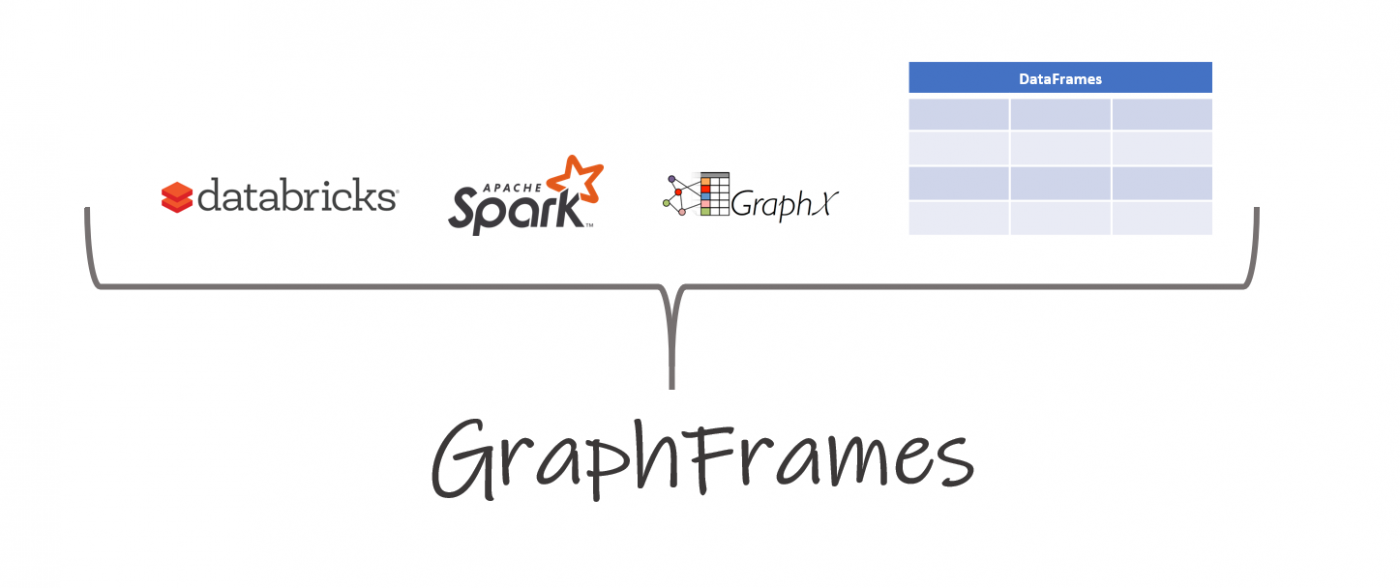
\includegraphics[width=.7\linewidth]{img/8-1_graphframes.png}
    \caption[Stack of the different technologies we are using for the second solution]{Stack of the different technologies we are using for the second solution\footnotemark}
\end{figure}

\footnotetext{\url{https://adatis.co.uk/graphframes/}}

\subsection{GraphFrames}

As it name goes, GraphFrame is a package for Apache Spark providing support for DataFrame-based Graphs. According to the introductory lines, the main goal of this stage of the development was to move our solution one step further in the abstraction level, from a solution based on RDDs to another based on DataFrames. From the ground up, we always believed RDDs weren't the go-to. What's more, RDDs are discouraged as they seem to be outdated in comparison to DataFrames and Datasets. More into this will be discussed in the next section.

\subsection{DataFrames and Datasets}

From Spark version 1.3 onwards, what were once known as SchemaRDDs are now referred to as DataFrames. That may give us an idea of what a DataFrame is. In that sense, they basically are RDDs provided some Schema for the data that is collected. With the help of this schema, DataFrames may be seen as rows with uniform structure: columns. Whereas RDDs are more akin to objects, DataFrames are closer to a table in a data base. This is quite relevant, as managing schemas to describe data allows us to perform operations over data in a much more efficient way than using Java serialization. It is worth mentioning that from Spark version 2.0 onwards, DataFrames can be understood as a type alias for \texttt{Dataset[Row]}, as they merged both APIs. In that sense, Datasets can be seen as the combination of the best from both worlds: with the appearance of a Java object from the outside, but with the shape of a table in RDBMS internally.

We now have a clear vision of what a DataFrame is. The problem is that even though they provide some nice features for data wrangling: schemas allow us to establish contracts so consumers know exactly the shape of the data they are working with, they are not so nicely implemented currently. Not only Apache Spark has no official support for working with DataFrame-based Graphs: notice GraphFrames is required, but the variety of supported types is scarce: including primitive types and Dates. Long has been discussed in this sense, but nothing has really changed since 2015\footnote{\url{https://issues.apache.org/jira/browse/SPARK-7768}}. To clarify this, let's put it into perspective.

\subsubsection{Encoders and User-defined Types}

Working with simple data-structures is a trivial task in Apache Spark. What is not so easy to handle are custom data types. If the DataFrame cannot implicitly retrieve an Encoder, the user will be required to provide one. This is needed for Spark SQL to infer the schemas of the data we are working with. The complex the data-structure, the harder it is for the programmer to write an appropriate serialization/deserialization mechanism. Notice how this solution is far from efficient as it is based on serialization for data storage and retrieval, something we were trying to fix from the RDD-based solution. Another possibility could be writing your own User-defined type, which can be understood as a wrapper for the actual type. However, the amount of boiler-plate code needed, and the complexity of the data to be stored prevents us from writing an appropriate solution. More into this will be discussed in the following paragraphs.

As we have mentioned earlier, two main possible solutions arise for the problem of handling complex data: \textit{Custom encoders} and \textit{User-defined types}. It is a requirement for this solution not only to handle complex data, but unsupported, as we are not only trying to store complex data structures, but types that are not currently supported by the DataFrame API. This is a crucial argument against this DataFrame-based solution as we need to store URLs, which aren't supported by Spark SQL. The problem is that both of the mentioned solutions are inefficient. First, collection Encoders tend to act as bottlenecks in terms of performance. To follow up on this, storing non-standard objects in Spark is a mess\footnote{\url{https://stackoverflow.com/questions/36648128/how-to-store-custom-objects-in-dataset}}. The current situation of the Framework basically supports primitive types and not so complex case classes. What's more, objects are serialized using \texttt{kryo} encoder which stores them as flat binary objects, losing some information and preventing us from using operations like \texttt{join}. Needed for Pregel to work. Thus, a custom, complex and inefficient encoder or type is not the solution we need. See figure \ref{fig:wikibaseClassDiagram} for an expanded description of the data model we are working with.

\begin{figure}[ht]
    \centering
    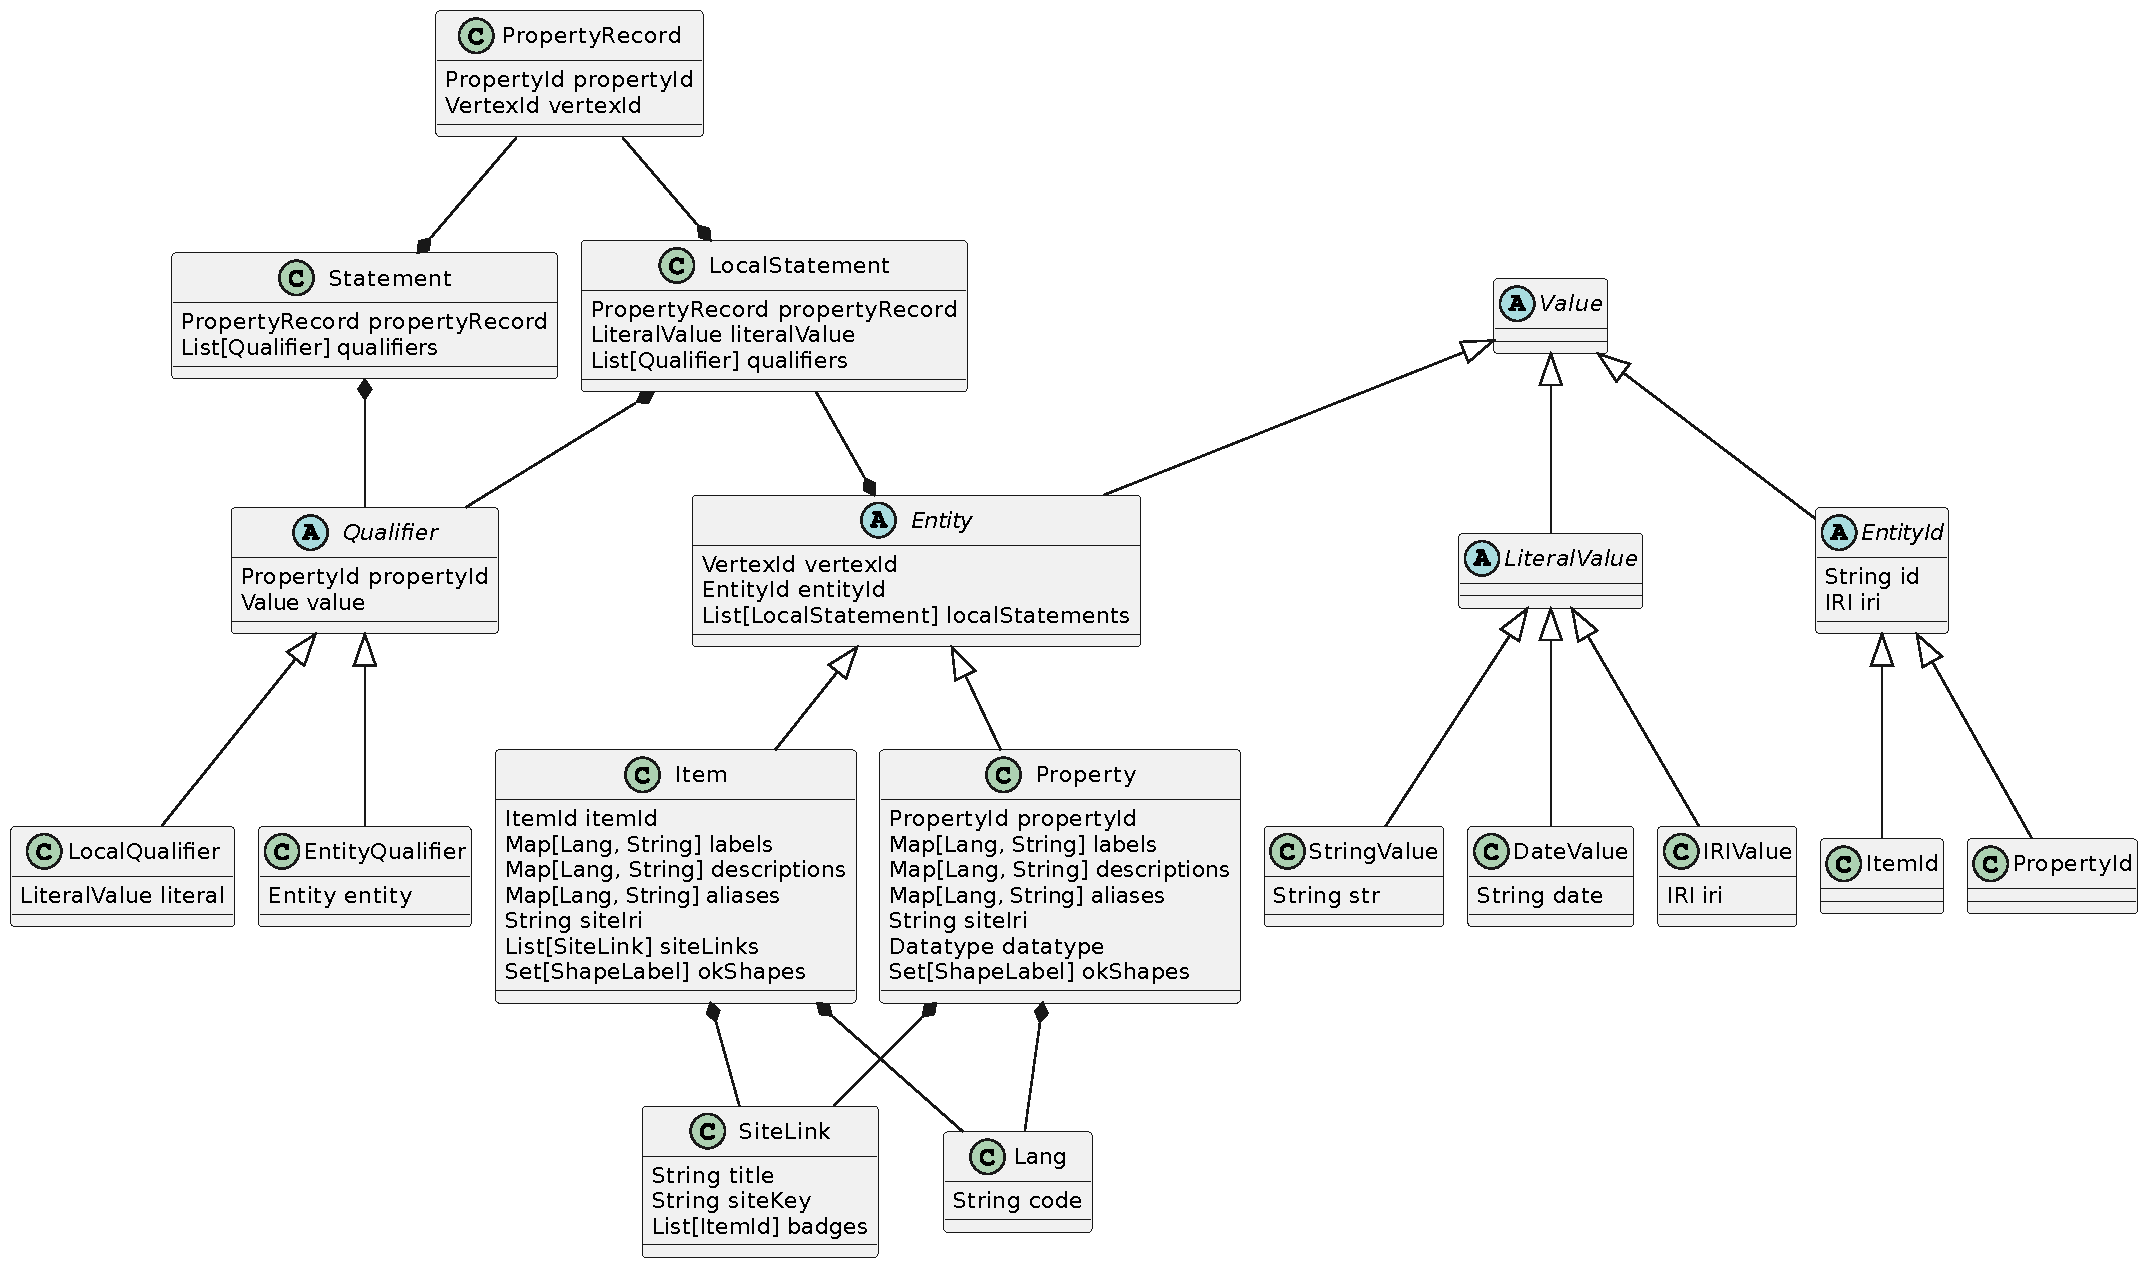
\includegraphics[width=\textwidth]{diagrams/8-1_wikibaseClassDiagram.pdf}
    \caption[Class diagram of the Wikibase data model as implemented in WShEx]{Class diagram of the Wikibase data model as implemented in WShEx\footnotemark}
    \label{fig:wikibaseClassDiagram}
\end{figure}
\footnotetext{\url{https://github.com/weso/shex-s}}

As a remark, it is worth noting that the code implementing the User-defined types for the data model above has a length of around 700 lines of code. While the actual algorithm takes around 100 lines of code to be written. For us to understand this, we have to describe how the so-called User-defined types are implemented in Apache Spark.


\begin{code}[User-defined types as implemented in Apache Spark]
    \inputminted{scala}{code/listings/8-1_udt.scala}
\end{code}

As noted in the first line of the above example, the description of user-defined types is annotated as an unstable API meant for developers. This implies that in minor Spark versions, the API may change or be eliminated. The use of it is at the user's own risk. As a consequence, if we use this approach, we will end up with an unstable solution. Not only that, but the processes for serializing and deserializing, along with the SQL schema -- which is no longer inferred by Scala's reflection system -- should be explicitly defined. Having said that, after we've specified what we've covered above, we're only establishing the wrapper, and yet no relationship is established between the real object and the User-defined type in the eyes of Spark's engine. To deal with this, we have two options: annotating the class we want to encapsulate or explicitly registering it. The former requires that the programmer has access to the class being wrapped. An ineffective technique that has been superseded by the latter since Spark 2.0. What's striking here is that it took Spark developers 6 years to come up with an answer in this regard. The API for user-defined types is essentially unmaintained, and dealing with custom objects in Spark is the framework's weak point. More on this was covered in the previously mentioned issue\footnote{\url{https://issues.apache.org/jira/browse/SPARK-7768}}.

\begin{code}[Registration of an User-defined type in Apache Spark]
    \inputminted{scala}{code/listings/8-2_udtRegistration.scala}
\end{code}

\subsubsection{The Catalyst Optimizer}

\section{Implementation of the Second Pregel solution}

\chapter{Third Pregel solution}
\label{chapter:third}
\epigraph{\textit{The most damaging phrase in the English language is "we have always done it this way".}}{-- \textup{Grace Hopper}}

\section{Technology stack}

\begin{figure}[ht]
    \begin{subfigure}[c]{.45\textwidth}
        \centering
        
\includegraphics[width=.7\linewidth]{img/9-1_rust.jpg}
        \caption{Rust programming language}
    \end{subfigure}%
    \hspace*{0.5em}
    \begin{subfigure}[c]{.45\textwidth}
        \centering
        
\includegraphics[width=.7\linewidth]{img/9-2_duckdb.png}
        \caption{DuckDB}
    \end{subfigure}%
    \caption{Stack of the different technologies we are using for the third solution}
\end{figure}

\chapter{Experimental Procedure}
\label{chapter:experiment}
\input{thesis_10_experiment}

\part{Project Synthesis}

\chapter{Results and Analysis}
\label{chapter:results}
\input{thesis_11_results}

\chapter{Planning and Budget}
\label{chapter:planning}
\begin{figure}[ht]
    \centering
    \includestandalone[width=1\textwidth]{diagrams/12-1_timeline}
    \caption{Project timeline highlighting the most important reached milestones}
    \label{fig:timeline}
\end{figure}

\begin{table}[ht]
    \centering
    Second\documentclass{standalone}
\usepackage[table,xcdraw]{xcolor}
\usepackage{varioref,multicol}
\usepackage{hyperref}  
\begin{document}
\begin{tabular}{|r|llll|}
    \hline
    \rowcolor[HTML]{C0C0C0}
    \multicolumn{1}{|c|}{\cellcolor[HTML]{C0C0C0}\textbf{ID}}     & \multicolumn{1}{c|}{\cellcolor[HTML]{C0C0C0}\textbf{Task name}} & \multicolumn{1}{c|}{\cellcolor[HTML]{C0C0C0}\textbf{Duration}} & \multicolumn{1}{c|}{\cellcolor[HTML]{C0C0C0}\textbf{Start}} & \multicolumn{1}{c|}{\cellcolor[HTML]{C0C0C0}\textbf{Finish}} \\ \hline
    1                                                             & \multicolumn{4}{c|}{\textit{Meetings}}                                                                                                                                                                                                                        \\ \hline
    1.1                                                           & \multicolumn{1}{l|}{Project's first meeting}                    & \multicolumn{1}{l|}{1 hour}                                    & \multicolumn{1}{l|}{Fri 16 September, 2022}                 & Fri 16 September, 2022                                       \\ \hline
    1.2                                                           & \multicolumn{1}{l|}{Project's second meeting}                   & \multicolumn{1}{l|}{2.5 hours}                                 & \multicolumn{1}{l|}{Thu 29 September, 2022}                 & Thu 29 September, 2022                                       \\ \hline
    1.3                                                           & \multicolumn{1}{l|}{Project's third meeting}                    & \multicolumn{1}{l|}{2 hours}                                   & \multicolumn{1}{l|}{Mon 20 February, 2023}                  & Mon 20 February, 2023                                        \\ \hline
    2                                                             & \multicolumn{4}{c|}{\textit{Literature Review}}                                                                                                                                                                                                               \\ \hline
    2.1                                                           & \multicolumn{1}{l|}{Knowledge graphs}                           & \multicolumn{1}{l|}{5 hours}                                   & \multicolumn{1}{l|}{Thu 29 September, 2022}                 & Fri 30 September, 2022                                       \\ \hline
    2.2                                                           & \multicolumn{1}{l|}{Wikibase graphs}                            & \multicolumn{1}{l|}{10 hours}                                  & \multicolumn{1}{l|}{Fri 30 September, 2022}                 & Sat 15 October, 2022                                         \\ \hline
    2.3                                                           & \multicolumn{1}{l|}{Knowledge graph validation}                 & \multicolumn{1}{l|}{7 hours}                                   & \multicolumn{1}{l|}{Sat 29 October, 2022}                   & Sat 5 November, 2022                                         \\ \hline
    2.4                                                           & \multicolumn{1}{l|}{Knowledge graph Subsetting}                 & \multicolumn{1}{l|}{0.5 hours}                                 & \multicolumn{1}{l|}{Mon 7 November, 2022}                   & Mon 7 November, 2022                                         \\ \hline
    2.5                                                           & \multicolumn{1}{l|}{MapReduce}                                  & \multicolumn{1}{l|}{3 hours}                                   & \multicolumn{1}{l|}{Tue 4 October, 2022}                    & Tue 4 October, 2022                                          \\ \hline
    2.6                                                           & \multicolumn{1}{l|}{Pregel algorithm}                           & \multicolumn{1}{l|}{6 hours}                                   & \multicolumn{1}{l|}{Tue 4 October, 2022}                    & Thu 6 October, 2022                                          \\ \hline
    3                                                             & \multicolumn{4}{c|}{\textit{Dissertation Document}}                                                                                                                                                                                                           \\ \hline
    3.1                                                           & \multicolumn{1}{l|}{Introduction}                               & \multicolumn{1}{l|}{5 hours}                                   & \multicolumn{1}{l|}{Wed 9 November, 2022}                   &                                                              \\ \hline
    3.2                                                           & \multicolumn{1}{l|}{Related Work}                               & \multicolumn{1}{l|}{3 hours}                                   & \multicolumn{1}{l|}{Fri 11 November, 2022}                  &                                                              \\ \hline
    3.3                                                           & \multicolumn{1}{l|}{Theoretical Background}                     & \multicolumn{1}{l|}{45 hours}                                  & \multicolumn{1}{l|}{Thu 29 September, 2022}                 &                                                              \\ \hline
    3.4                                                           & \multicolumn{1}{l|}{Design of the Pregel solution}              & \multicolumn{1}{l|}{10 hours}                                  & \multicolumn{1}{l|}{Fri 11 November, 2022}                  &                                                              \\ \hline
    3.5                                                           & \multicolumn{1}{l|}{Experimental Procedure}                     & \multicolumn{1}{l|}{}                                          & \multicolumn{1}{l|}{}                                       &                                                              \\ \hline
    3.6                                                           & \multicolumn{1}{l|}{Results and Analysis}                       & \multicolumn{1}{l|}{}                                          & \multicolumn{1}{l|}{}                                       &                                                              \\ \hline
    3.7                                                           & \multicolumn{1}{l|}{Planning and Budget}                        & \multicolumn{1}{l|}{}                                          & \multicolumn{1}{l|}{Thu 20 October, 2022}                   &                                                              \\ \hline
    3.8                                                           & \multicolumn{1}{l|}{Conclusions}                                & \multicolumn{1}{l|}{}                                          & \multicolumn{1}{l|}{}                                       &                                                              \\ \hline
    4                                                             & \multicolumn{4}{c|}{\textit{Proposed Solution Development}}                                                                                                                                                                                                   \\ \hline
    4.1                                                           & \multicolumn{1}{l|}{Second Pregel solution}                     & \multicolumn{1}{l|}{30 hours}                                  & \multicolumn{1}{l|}{Sun 29 January, 2023}                   & Mon 20 February, 2023                                        \\ \hline
    4.2                                                           & \multicolumn{1}{l|}{Third Pregel solution}                      & \multicolumn{1}{l|}{}                                          & \multicolumn{1}{l|}{Tue 21 February, 2023}                  &                                                              \\ \hline
    5                                                             & \multicolumn{4}{c|}{\textit{Learning new technologies}}                                                                                                                                                                                                       \\ \hline
    5.1                                                           & \multicolumn{1}{l|}{Scala}                                      & \multicolumn{1}{l|}{10 hours}                                  & \multicolumn{1}{l|}{Tue 6 December, 2022}                   & Tue 27 December, 2022                                        \\ \hline
    5.2                                                           & \multicolumn{1}{l|}{Apache Spark}                               & \multicolumn{1}{l|}{5 hours}                                   & \multicolumn{1}{l|}{Thu 29 December, 2022}                  & Sat 7 January, 2023                                          \\ \hline
    5.3                                                           & \multicolumn{1}{l|}{Rust}                                       & \multicolumn{1}{l|}{5 hours}                                   & \multicolumn{1}{l|}{Tue 21 February, 2023}                  &                                                              \\ \hline
    \multicolumn{2}{|r|}{\cellcolor[HTML]{C0C0C0}\textbf{Total:}} & \multicolumn{1}{l|}{159 hours}                                                                                                                                                                                                                                \\ \cline{1-3}
\end{tabular}
\end{document}
    \caption{Tasks planning of the project}
    \label{tab:timeline}
\end{table}

\chapter{Conclusions}
\label{chapter:conclusions}
\input{thesis_13_conclusions}

\part{Annexes and References}

\chapterimage{img/misc/heading_bib.jpg} % Chapter heading image
\chapter{References} % Chapter heading image
\printbibliography[heading=bibempty]

\end{document}